% !TeX encoding = UTF-8
% !TeX root = MAIN.tex

\section{Introduction}
\subsection{Game Description}
	\label{sec:desc}
	Minesweeper is a popular puzzle video game.
	The game features a grid of $x \times y$ tiles. Hidden throughout that field are multiple mines which the player needs to avoid. The game ends in a win if the player manages to clear all fields without detonating a single bomb. (\cite{Minesweeper})
	
	Each tile within the grid can be either unopened, opened or flagged. Unopened tiles are blank and can be opened. Players are able to flag a cell to denote a possible mine location. Flagged cells are marked with a flag symbol on the grid and still considered as unopened. (\cite{Minesweeper})
	
	Selecting a cell opens it. An open cell can either be a mine, which immediately ends the game and results in failure, a number that indicates the amount of mines that are horizontally, vertically or diagonally adjacent to it, or blank, in which case all non-mine cells neighbouring it will be revealed. A cell can have up to eight neighbours. (\cite{Minesweeper})
	
	A game of Minesweeper begins by opening a cell. While playing, increasingly more information about the grid becomes known to the player which further aids in deducing the next safe cell to open. Furthermore, the remaining amount of mines is given to the player. The mine count is calculated by subtracting the total number of mines by the number of flagged cells, thus also allowing the mine count to be negative. (\cite{Minesweeper})
	
	To win at Minesweeper, the player has to clear all non-mine cells without opening a mine. There isn't a score count or time limit, however players' time to finish is being measured. Difficulty can be increased by adding more mines or starting with a larger game field.
	
	After establishing the game rules and restrictions, we define our language \textbf{MSWP}: A field is in \textbf{MSWP} if there exists a layout of bombs such that the game field is valid, i.e. the numbers in the game field correctly correspond to the amount of neighbouring bombs.
	
	% image source: https://www.gamepro.de/galerien/minesweeper,136622.html
	% src: wikipedia
	% consider using an image with a more open license
	% or create your own screenshot
	\begin{figure}[tp]
		\centering
		\fbox{\includegraphics[width=0.7\textwidth, keepaspectratio]{_img/minesweeper_game}}
		\caption{A game of Minesweeper \\
		Source: \cite{image}}
		\label{fig:game}
	\end{figure}
	
\subsection{Motivation}
	Choosing Minesweeper as this project's topic was appealing for a multitude of reasons. The primary ones of this paper are the wide-spread familiarity with the game and the topic being well-suited to the Computational Complexity lecture at JKU Linz.
	
	Since Minesweeper has been bundled with numerous operating systems, millions of users have become deeply acquainted with its gameplay. Thus this paper should be more accessible to readers of a non-technical background.

	To win at Minesweeper, players have to use logical reasoning to deduce which fields are safe and which are not. Such principals and strategies perfectly align with the subject matter covered in the lecture.
	
\section{NP membership of Minesweeper}
	In this section of the paper we want to show that \textbf{MSWP} is in the problem class \textbf{NP}. So there exists a short certificate and a verifier that accepts that certificate in at most polynomial time. If that is the case, then our language is complete. If the verifier also rejects assignment which are not part of the language, then it is sound as well (\cite{lecture}). Both of these requirements need to be fulfilled in order for our language to be part of \textbf{NP}.
	
	For Minesweeper specifically we have to consider a placement of $b$ on the game field $G$, such that every numbered cell correctly indicates the number of adjacent bombs (see section \ref{sec:rules} for all rules that need to be fulfilled).
	
\subsection{Certificate}
	The certificate in this case is a assignment of bombs to the game board grid, i.e. a configuration for each cell that tells us whether it's a bomb or not.
	
\subsection{Accepting and Rejecting}
	To correctly verify the certificate, we need to (i) check the number of bombs of the certificate aligns with the number of bombs $b$ of the input, (ii) for each numbered cell count the number of bombs in the neighbouring cells and verify that the count matches the value given in the cell.
	
	\textbf{MSWP} fulfills the completeness criteria of \textbf{NP}, as if there is a Minesweeper game $MG \in \text{\textbf{MSWP}}$, then a board configuration with $b$ bombs exists, where all numbered cells are consistent with the count of neighbouring bombs. Using this board placement as a certificate, the verifier will accept since all verification rules are fulfilled. As our input consists of the game field width $n$, game field height $m$ and amount of bombs $b$ (so $(n \cdot m) + 1$), the input size is at most polynomial ($O(n \cdot m)$). In the worst case (square grid, $n = m$) our runtime is $O(n^2)$.
	
	The soundness of \textbf{MSWP} is present as well, because we reject every certificate that violates the game field rules set by us (see section \ref{sec:rules}). Thus it is not possible for a false certificate to be accepted.
	
	As we have proven \textbf{MSWP} is complete and sound, thus we conclude that \textbf{MSWP} is a member of \textbf{NP}.
	
	
\subsection{Encoding Minesweeper}
	Because of the relative simplicity and structured rule set of Minesweeper, we can construct logical formula based on those rules.
	
	\paragraph{Input}
	Because Minesweeper is played on a two-dimensional field, we have the game board width $n$ and height $m$. Furthermore we also have the number of bombs $b$.
	
	\paragraph{Output}
	We want to know if the given configuration is a valid assignment of bombs.
	
	\paragraph{Game Board Definition}
	To effectively encode the game board, we assign a unique label $F_iX$ to each cell on the game board. $i$ is a natural number refers to a specific cell on the board. We start at the cell on the left-most upper corner of the game field and start counting up. $i \in \{1, \ldots, n \cdot m\}$.
	
	$X$ on the other hand specifies the amount of bombs that surround the current cell $F_i$. $X$ ranges from $0$ to $9$, however we have chosen $9$ to mean that a bomb is placed on that specific position. $X \in \{\underbrace{0,1,2,3,4,5,6,7,8}_{\text{neighbouring bombs}}, \underbrace{9}_{\text{bomb}}\}$.
	
	\paragraph{Neighbours}
	As previously established, a cell can have up to $k=8$ neighbours.
	We encode each neighbour of the current cell $F_i$ by $n_k$ where $k \in \{1, \ldots, 8\}$. Each $n_k$ has a truth value. If $n_k$ is true, then that neighbour is a bomb. If it is false, then the neighbour isn't a bomb. We introduce this for easier notation when iterating over the neighbours.
	
\subsection{Game Rules} \label{sec:rules}
	\paragraph{Rule: Each field has at least one value}
	
	{\Large
		\begin{center}
			$\mathop{\bigwedge}\limits_{i = 1}^{n \cdot m} (\mathop{\bigvee}\limits_{x=0}^{9} F_{i}X)$
		\end{center}
	}	
	
	\paragraph{Rule: each field has at most one value}
	
	{\Large
		\begin{center}
			$\mathop{\bigwedge}\limits_{i = 1}^{n \cdot m} \ \mathop{\bigwedge}\limits_{0 \leq x_1 < x_2 \leq 9} \ (\overline{F_{ij}X_1} \lor \overline{F_{ij}X_2)}$
		\end{center}	
	}

	
	\paragraph{Rule: across the entire game board there are at least $b$ bombs}
	
	\begin{center}
		$j = n \cdot m - b + 1$ \\
		$\binom{n \cdot m}{j} \text{ clauses}$ \\
		$j \text{ literals each}$
	\end{center}
	
	{\Large
		\begin{center}
			$\mathop{\land}\limits_{1 \leq i_1 < i_2 < \ldots < ij \leq n \cdot m} \ (F_{i1}9 \lor F_{i2}9 \lor \ldots \lor F_{ij}9)$
		\end{center}
	}
	
	\paragraph{Rule: across the entire game board there are at most $b$ bombs}
	
	\begin{center}
		$ \binom{n \cdot m}{b+1}$ clauses \\
		$b+1$ literals each
	\end{center}
	
	{\Large
		\begin{center}
			$\mathop{\bigwedge}\limits_{1 \leq i_1 < i_2 < \ldots < ib < ib+1 \leq n \cdot m} \ (\overline{F_{i1}9} \lor \overline{F_{i2}9} \lor \ldots \lor \overline{F_{ib}9} \lor \overline{F_{ib+1}9})$
		\end{center}
	}

	\paragraph{Rule: if a field has value 0, then no neighbours are a bomb}
	
	\begin{center}
		$n \cdot m \cdot 8$ clauses \\
		$2$ literals each	
	\end{center}
	
	{\Large
		\begin{center}
			$\mathop{\bigwedge}\limits_{i = 1}^{n \cdot m} \ \mathop{\bigwedge}\limits_{k = 1}^{8} \ (\overline{F_{i}0} \lor \overline{n_k})$
		\end{center}
	}
	
	\paragraph{Rule: if a field has value $z$, then exactly $z$ neighbours are bombs}
	
	\begin{center}
		$1 \leq z \leq 7$
	\end{center}
	
	
	\textbf{at least $z$ bombs}:
	
	\begin{center}
		$j = 8 - z + 1$ \\
		$n \cdot m \cdot \binom{8}{j}$ clauses \\
		$j+1$ literals each
	\end{center}
	
	{\Large
		\begin{center}
			$\mathop{\bigwedge}\limits_{i = 1}^{n \cdot m} \ \mathop{\bigwedge}\limits_{1 \leq k_1 < k_2 < \ldots < kj \leq 8} \ (\overline{F_{i}X} \lor n_{k1} \lor \ldots \lor n_{kj})$
		\end{center}
	}
	
	\textbf{at most $z$ bombs}:
	
	\begin{center}
		$j = z + 1$ \\ 
		$n \cdot m \cdot \binom{8}{j}$ clauses \\ 
		$j+1$ literals each
	\end{center}
	
	{\Large
		\begin{center}
			$\mathop{\bigwedge}\limits_{i = 1}^{n \cdot m} \ \mathop{\bigwedge}\limits_{1 \leq k_1 < k_2 < \ldots < kj \leq 8} \ (\overline{F_{i}X} \lor \overline{n_{k1}} \lor \ldots \lor \overline{n_{kj}})$
		\end{center}
	}
	
	\paragraph{Rule: if a field has value 8, then all neighbours are a bombs}
	
	\begin{center}
		$n \cdot m \cdot 8$ clauses \\
		$2$ literals each \\
	\end{center}
	
	{\Large
		\begin{center}
			$\mathop{\bigwedge}\limits_{i = 1}^{n \cdot m} \ \mathop{\bigwedge}\limits_{k = 1}^{8} \ (\overline{F_{i}8} \lor n_k)$
		\end{center}
	}
	

\section{Karp Reduction from 3-SAT}
	\subsection{SAT $\leq_p$ MSWP}
	To encode a \textbf{SAT} formula \textit{F} with \textit{n} variables and \textit{m} clauses into an instance of \textbf{MSWP} \textit{M}, we define structures which function as building blocks. (see section \ref{sec:comp}).
	
	The basic idea is to look closer at the rows and columns. Each row of the game board represents a clause, while each column is a stream of inputs and variables where we determine the value for each variable. Via these two stream and our defined components we construct a formula in CNF that is satisfiable if and only if there exists a layout of bombs such that the Minesweeper board is in a valid configuration.
	
	\begin{figure}[h!]
		\centering
		\scalebox{1.1}{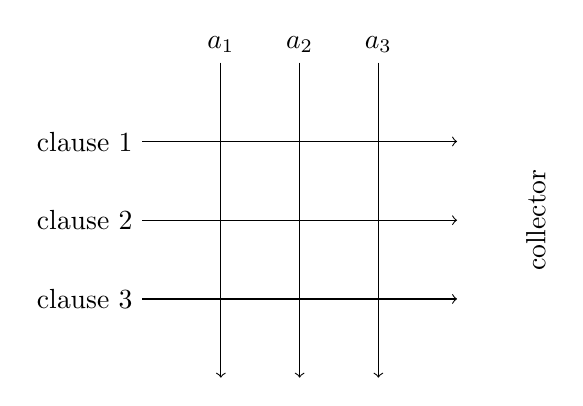
\begin{tikzpicture}
\draw[->] (-3,3) node[anchor=south]{\(a_1\)} -- (-3,-1);
\draw[->] (-2,3) node[anchor=south]{\(a_2\)} -- (-2,-1);
\draw[->] (-1,3) node[anchor=south]{\(a_3\)} -- (-1,-1);
\draw[->] (-4,2) node[anchor=east]{clause 1} -- (0,2);
\draw[->] (-4,1) node[anchor=east]{clause 2} -- (0,1);
\draw[->] (-4,0) node[anchor=east]{clause 3} -- (0,0);
\node[rotate=90] at (1,1) {collector};
\end{tikzpicture}}
		\caption{Concept behind \textbf{MSWP} formula construction}
		\label{fig:idea}
	\end{figure} 

	\subsection{Alphabet \& Notation}
	First of all we introduce an alphabet that will help us later with the verification. The alphabet encodes all possible values a cell within the game field may have. A cell could be number $n$ without zero (same behaviour as in Minesweeper), be blank (defined here as $0$), have a predefined bomb, an input-dependent bomb, an input-dependent safe cell, a variable (unopened cell) or a cell without a value. Basically we define $\alpha = \{n, 0, \cdot, \textcolor{red}{\cdot}, \textcolor{red}{\times}, \textcolor{green}{?}, \textcolor{green}{\cdot}\}$.

	As the following chapters will frequently use the alphabet in multiple figures, we created a reference table for the readers' convenience.

	\begin{table}
		\begin{tabular}{|c|c|} \hline
			\rowcolor{cyan}\textbf{Symbol} & \textbf{Definition} \\ \hline
			$n$ & denotes how many bombs are in the neighbourhood of cell \\ \hline
			$0$ & blank cell \\ \hline
			
\begin{tikzpicture}\fill[color=black] circle (4pt);\end{tikzpicture} & predefined bombs \\ \hline
			
\begin{tikzpicture}\fill[color=red] circle (4pt);\end{tikzpicture} & input-dependent bomb \\ \hline
			\begin{tikzpicture}[baseline=(n.base)]\node[color=red] (n) {X};\end{tikzpicture} & input-dependent safe cell \\ \hline
			\begin{tikzpicture}[baseline=(n.base)]\node[color=green!70!black] (n) {\textbf{?}};\end{tikzpicture} & value of variable (can be true: \begin{tikzpicture}[baseline=(n.base)]\node[color=red] (n) {X};\end{tikzpicture} or false: 
\begin{tikzpicture}\fill[color=red] circle (4pt);\end{tikzpicture}) \\ \hline
			
\begin{tikzpicture}\fill[color=green!70!black] circle (2pt);\end{tikzpicture} & input-dependent cell (can become \begin{tikzpicture}[baseline=(n.base)]\node[color=red] (n) {X};\end{tikzpicture} or 
\begin{tikzpicture}\fill[color=red] circle (4pt);\end{tikzpicture} depending on variable value) \\ \hline
		\end{tabular}
		\caption{Notation Table} \label{tbl:notation}
	\end{table}

	\subsection{Evaluation}
	The method to compute our Minesweeper field into a logical formula goes as such:
	\begin{itemize}
		\item We divide the game field into rows and columns
		\item We form clauses via the rows, by going from left to right
		\item We compute variables by going from top to bottom for each column
		\item To aid with our computation, we use the help of multiple components which alter the input stream of our rows and columns
	\end{itemize} 

	\subsection{Components} \label{sec:comp}
	
	
	\paragraph{\textsc{\textbf{Input Stream}}}
	This input stream goes from top to bottom and evaluates each variable (\begin{tikzpicture}[baseline=(n.base)]\node[color=green!70!black] (n) {\textbf{?}};\end{tikzpicture} and 
\begin{tikzpicture}\fill[color=green!70!black] circle (2pt);\end{tikzpicture}) and sets its according value (\begin{tikzpicture}[baseline=(n.base)]\node[color=red] (n) {X};\end{tikzpicture} or 
\begin{tikzpicture}\fill[color=red] circle (4pt);\end{tikzpicture}). (See Table \ref{tbl:notation})
	
	\begin{figure}[H]
		\centering
		\scalebox{0.8}{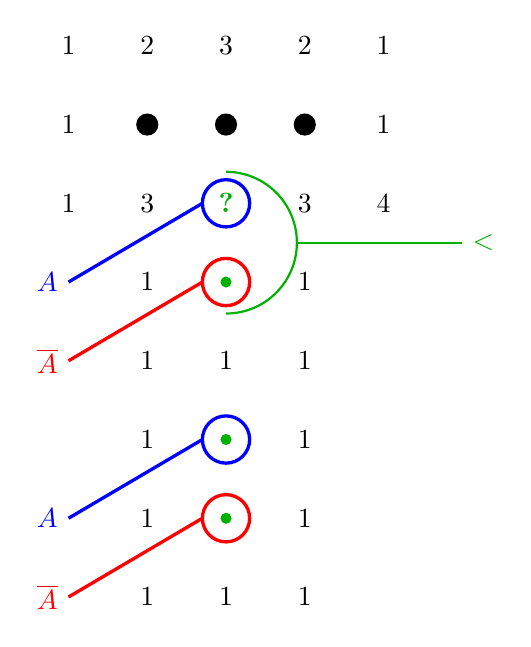
\begin{tikzpicture}
    \node at (0,0) {1};
    \node at (1,0) {2};
    \node at (2,0) {3};
    \node at (3,0) {2};
    \node at (4,0) {1};
    
    \node at (0,-1) {1};
    \fill (1,-1) circle (4pt);
    \fill (2,-1) circle (4pt);
    \fill (3,-1) circle (4pt);
    \node at (4,-1) {1};
    
    \node at (0,-2) {1};
    \node at (1,-2) {3};
    \node[color=green!70!black] at (2,-2) {\textbf{?}};
    \draw[blue, very thick] (2,-2) circle [radius=0.3] (1.7,-2) -- (0,-3) node[anchor=east] {\(A\)};
    \node at (3,-2) {3};
    \node at (4,-2) {4};


    \draw[thick, green!70!black] (2,-1.6) arc[start angle=90, end angle=-90, radius=0.9];
    
    \draw[thick, green!70!black](2.9,-2.5) -- (5,-2.5) node[anchor=west]{\(<\)};
    
    \node at (1,-3) {1};
    \fill[color=green!70!black] (2,-3) circle (2pt);
    \draw[red, very thick] (2,-3) circle [radius=0.3] (1.7,-3) -- (0,-4) node[anchor=east] {\(\overline A\)};
    \node at (3,-3) {1};
    
    \node at (1,-4) {1};
    \node at (2,-4) {1};
    \node at (3,-4) {1};

    \node at (1,-5) {1};
    \fill[color=green!70!black] (2,-5) circle (2pt);
    \draw[blue, very thick] (2,-5) circle [radius=0.3] (1.7,-5) -- (0,-6) node[anchor=east] {\(A\)};
    \node at (3,-5) {1};

    \node at (1,-6) {1};
    \fill[color=green!70!black] (2,-6) circle (2pt);
    \draw[red, very thick] (2,-6) circle [radius=0.3] (1.7,-6) -- (0,-7) node[anchor=east] {\(\overline A\)};
    \node at (3,-6) {1};

    \node at (1,-7) {1};
    \node at (2,-7) {1};
    \node at (3,-7) {1};
\end{tikzpicture}}

		\begin{minipage}{0.48\textwidth}
			\centering
			\scalebox{0.6}{\input{graphics/input_stream_var_true}}
			\caption*{(a) true input}
		\end{minipage}
		\hfill
		\begin{minipage}{0.48\textwidth}
			\centering
			\scalebox{0.6}{\begin{tikzpicture}
    \node at (0,0) {1};
    \node at (1,0) {2};
    \node at (2,0) {3};
    \node at (3,0) {2};
    \node at (4,0) {1};
    
    \node at (0,-1) {1};
    \fill (1,-1) circle (4pt);
    \fill (2,-1) circle (4pt);
    \fill (3,-1) circle (4pt);
    \node at (4,-1) {1};
    
    \node at (0,-2) {1};
    \node at (1,-2) {3};
    \fill[color=red] (2,-2) circle (4pt);
    \node at (3,-2) {3};
    \node at (4,-2) {4};


    
    \node at (1,-3) {1};
    \node[color=red] at (2,-3) {\textbf{X}};
    \node at (3,-3) {1};
    
    \node at (1,-4) {1};
    \node at (2,-4) {1};
    \node at (3,-4) {1};

    \node at (1,-5) {1};
    \fill[color=red] (2,-5) circle (4pt);
    \node at (3,-5) {1};

    \node at (1,-6) {1};
    \node[color=red] at (2,-6) {\textbf{X}};
    \node at (3,-6) {1};

    \node at (1,-7) {1};
    \node at (2,-7) {1};
    \node at (3,-7) {1};
\end{tikzpicture}}
			\caption*{(b) false input}
		\end{minipage}
		
		\caption{Input Stream}
		\label{fig:inputstream}
	\end{figure} 

	\paragraph{\textsc{\textbf{Clause Stream}}}
	Represent a clause within our formula. It starts out as false. When we encounter a variable we check its truth value. If it evaluates to true, then our clause becomes true. Should the variable be false, but the clause's previous state was true, then the clause still stays true.
	So we use a logical or on the clause itself and the variable in the input stream $\underbrace{(x \lor y \lor \ldots)}_{\text{Clause}} \lor x$.

	In simple terms: The Clause Stream "carries" the state of the clause from left to right, and as soon as an input satisfies the clause, the clause becomes true for the rest of the stream.
	
	\begin{figure}[H]
		\centering
		\scalebox{1.2}{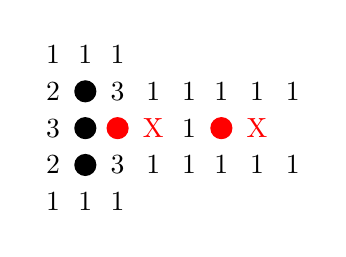
\begin{tikzpicture}
\usetikzlibrary {matrix}
    \newcommand{\redDot}{
        \fill[color=red] circle (4pt);
    }
    \newcommand{\redX}{
        \node[color=red] {X};
    }
    \newcommand{\blackDot}{
        \fill[color=black] circle (4pt);
    }
  \matrix[
  matrix of nodes,nodes={anchor=center}
]
  {
    1&1&1&&&&& \\
    2&\blackDot&3&1&1&1&1&1 \\
    3&\blackDot&\redDot&\redX&1&\redDot&\redX& \\
    2&\blackDot&3&1&1&1&1&1 \\
    1&1&1&&&&& \\
  };


\end{tikzpicture}}
		\caption{Clause Stream}
		\label{fig:clausestream}
	\end{figure} 

	\paragraph{\textsc{\textbf{Crossing}}}
	This is used when the Clause Stream and input stream meet, but the variable of the Input Stream is not part of the clause. This component causes for the variable in the Input Stream to be ignored by the Clause Stream, i.e. the Clause Stream will not use the variable. The Clause Stream and Input Stream remain unchanged.
	
	\begin{figure}[H]
		\centering
		\scalebox{0.8}{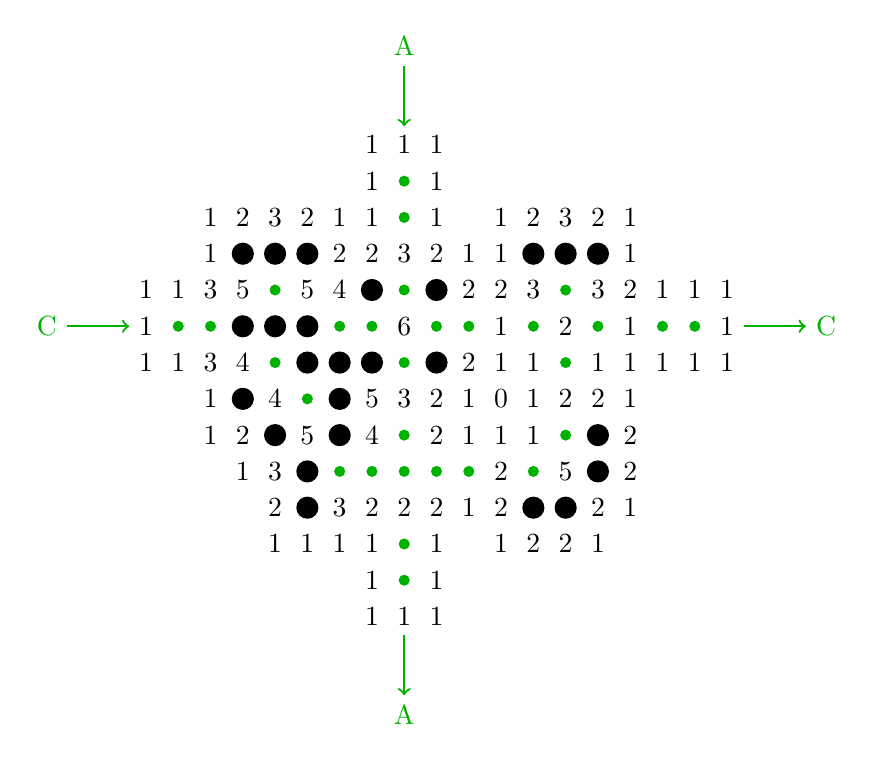
\begin{tikzpicture}
\usetikzlibrary {matrix}
    \newcommand{\greenDot}{
        \fill[color=green!70!black] circle (2pt);
    }
    \newcommand{\blackDot}{
        \fill[color=black] circle (4pt);
    }
  \matrix[
  matrix of nodes,nodes={anchor=center}
]
  {
    &&&&&&&1&|(north)|1&1&&&&&&&&& \\
    &&&&&&&1&\greenDot&1&&&&&&&&& \\
    &&1&2&3&2&1&1&\greenDot&1&&1&2&3&2&1&&& \\
    &&1&\blackDot&\blackDot&\blackDot&2&2&3&2&1&1&\blackDot&\blackDot&\blackDot&1&&& \\
    1&1&3&5&\greenDot&5&4&\blackDot&\greenDot&\blackDot&2&2&3&\greenDot&3&2&1&1&1 \\
    |(west)|1&\greenDot&\greenDot&\blackDot&\blackDot&\blackDot&\greenDot&\greenDot&6&\greenDot&\greenDot&1&\greenDot&2&\greenDot&1&\greenDot&\greenDot&|(east)|1 \\
    1&1&3&4&\greenDot&\blackDot&\blackDot&\blackDot&\greenDot&\blackDot&2&1&1&\greenDot&1&1&1&1&1 \\
    &&1&\blackDot&4&\greenDot&\blackDot&5&3&2&1&0&1&2&2&1&&& \\
    &&1&2&\blackDot&5&\blackDot&4&\greenDot&2&1&1&1&\greenDot&\blackDot&2&&& \\
    &&&1&3&\blackDot&\greenDot&\greenDot&\greenDot&\greenDot&\greenDot&2&\greenDot&5&\blackDot&2&&& \\
    
    &&&&2&\blackDot&3&2&2&2&1&2&\blackDot&\blackDot&2&1&&& \\

    &&&&1&1&1&1&\greenDot&1&&1&2&2&1&&&& \\
    &&&&&&&1&\greenDot&1&&&&&&&&& \\
    &&&&&&&1&|(south)|1&1&&&&&&&&& \\
  };

\draw[thick, color=green!70!black, ->] (east) -- ++(1,0) node[anchor=west] {C};
\draw[thick, color=green!70!black, <-] (west) -- ++(-1,0) node[anchor=east] {C};
\draw[thick, color=green!70!black, <-] (north) -- ++(0,1) node[anchor=south] {A};
\draw[thick, color=green!70!black, ->] (south) -- ++(0,-1) node[anchor=north] {A};

\end{tikzpicture}}
		\caption{Crossing}
		\label{fig:crossing}
	\end{figure}
	
	\begin{figure}[H]
		\centering
		\begin{tabular}{cc}
			\scalebox{0.6}{\input{graphics/crossing-a-false-c-false}} &
			\scalebox{0.6}{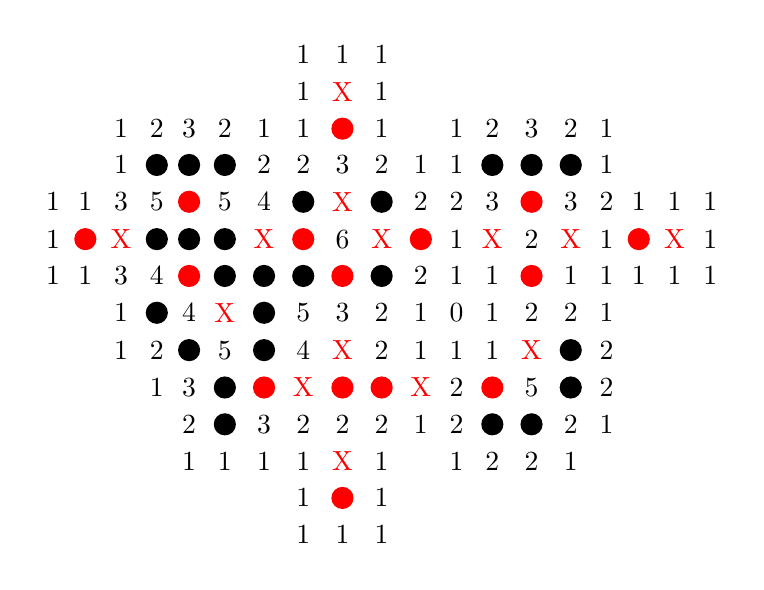
\begin{tikzpicture}
\usetikzlibrary {matrix}
    \newcommand{\redDot}{
        \fill[color=red] circle (4pt);
    }
    \newcommand{\redX}{
        \node[color=red] {X};
    }

    \newcommand{\blackDot}{
        \fill[color=black] circle (4pt);
    }
  \matrix[
  matrix of nodes,nodes={anchor=center}
]
  {
    &&&&&&&1&1&1&&&&&&&&& \\
    
    &&&&&&&1&\redX&1&&&&&&&&& \\
    
    &&1&2&3&2&1&1&\redDot&1&&1&2&3&2&1&&& \\
    &&1&\blackDot&\blackDot&\blackDot&2&2&3&2&1&1&\blackDot&\blackDot&\blackDot&1&&& \\
    
    1&1&3&5&\redDot&5&4&\blackDot&\redX&\blackDot&2&2&3&\redDot&3&2&1&1&1 \\
    1&\redDot&\redX&\blackDot&\blackDot&\blackDot&\redX&\redDot&6&\redX&\redDot&1&\redX&2&\redX&1&\redDot&\redX&1 \\
    1&1&3&4&\redDot&\blackDot&\blackDot&\blackDot&\redDot&\blackDot&2&1&1&\redDot&1&1&1&1&1 \\
    
    &&1&\blackDot&4&\redX&\blackDot&5&3&2&1&0&1&2&2&1&&& \\
    
    &&1&2&\blackDot&5&\blackDot&4&\redX&2&1&1&1&\redX&\blackDot&2&&& \\
    
    &&&1&3&\blackDot&\redDot&\redX&\redDot&\redDot&\redX&2&\redDot&5&\blackDot&2&&& \\
    
    &&&&2&\blackDot&3&2&2&2&1&2&\blackDot&\blackDot&2&1&&& \\

    &&&&1&1&1&1&\redX&1&&1&2&2&1&&&& \\
    
    &&&&&&&1&\redDot&1&&&&&&&&& \\
    
    &&&&&&&1&1&1&&&&&&&&& \\
  };



\end{tikzpicture}} \\[1em]
			\scalebox{0.6}{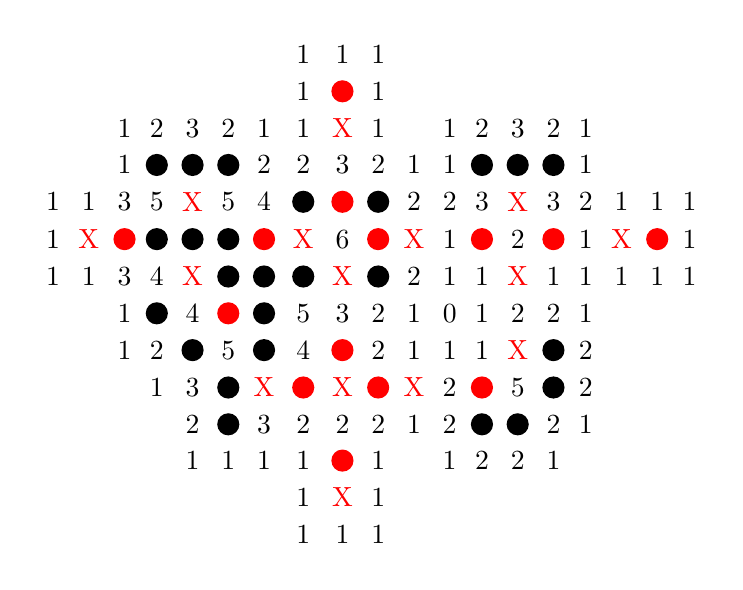
\begin{tikzpicture}
\usetikzlibrary {matrix}
    \newcommand{\redDot}{
        \fill[color=red] circle (4pt);
    }
    \newcommand{\redX}{
        \node[color=red] {X};
    }
    \newcommand{\blackDot}{
        \fill[color=black] circle (4pt);
    }
  \matrix[
  matrix of nodes,nodes={anchor=center}
]
  {
    &&&&&&&1&1&1&&&&&&&&& \\
    &&&&&&&1&\redDot&1&&&&&&&&& \\
    &&1&2&3&2&1&1&\redX&1&&1&2&3&2&1&&& \\
    &&1&\blackDot&\blackDot&\blackDot&2&2&3&2&1&1&\blackDot&\blackDot&\blackDot&1&&& \\
    
    1&1&3&5&\redX&5&4&\blackDot&\redDot&\blackDot&2&2&3&\redX&3&2&1&1&1 \\
    1&\redX&\redDot&\blackDot&\blackDot&\blackDot&\redDot&\redX&6&\redDot&\redX&1&\redDot&2&\redDot&1&\redX&\redDot&1 \\
    1&1&3&4&\redX&\blackDot&\blackDot&\blackDot&\redX&\blackDot&2&1&1&\redX&1&1&1&1&1 \\
    
    &&1&\blackDot&4&\redDot&\blackDot&5&3&2&1&0&1&2&2&1&&& \\
    
    &&1&2&\blackDot&5&\blackDot&4&\redDot&2&1&1&1&\redX&\blackDot&2&&& \\
    &&&1&3&\blackDot&\redX&\redDot&\redX&\redDot&\redX&2&\redDot&5&\blackDot&2&&& \\
    
    &&&&2&\blackDot&3&2&2&2&1&2&\blackDot&\blackDot&2&1&&& \\

    &&&&1&1&1&1&\redDot&1&&1&2&2&1&&&& \\
    &&&&&&&1&\redX&1&&&&&&&&& \\
    &&&&&&&1&1&1&&&&&&&&& \\
  };


\end{tikzpicture}} &
			\scalebox{0.6}{\input{graphics/crossing-a-true-c-true}}
		\end{tabular}
		\caption{Every possible assignment Clause Stream and Input Stream within Crossing. From top-left to bottom right the options are (Input, Clause): (false, false), (true,false), (false, true), (true, true)}
		\label{fig:crossingassignments}
	\end{figure}
	
	\begin{figure}[H]
		\centering
		\scalebox{0.7}{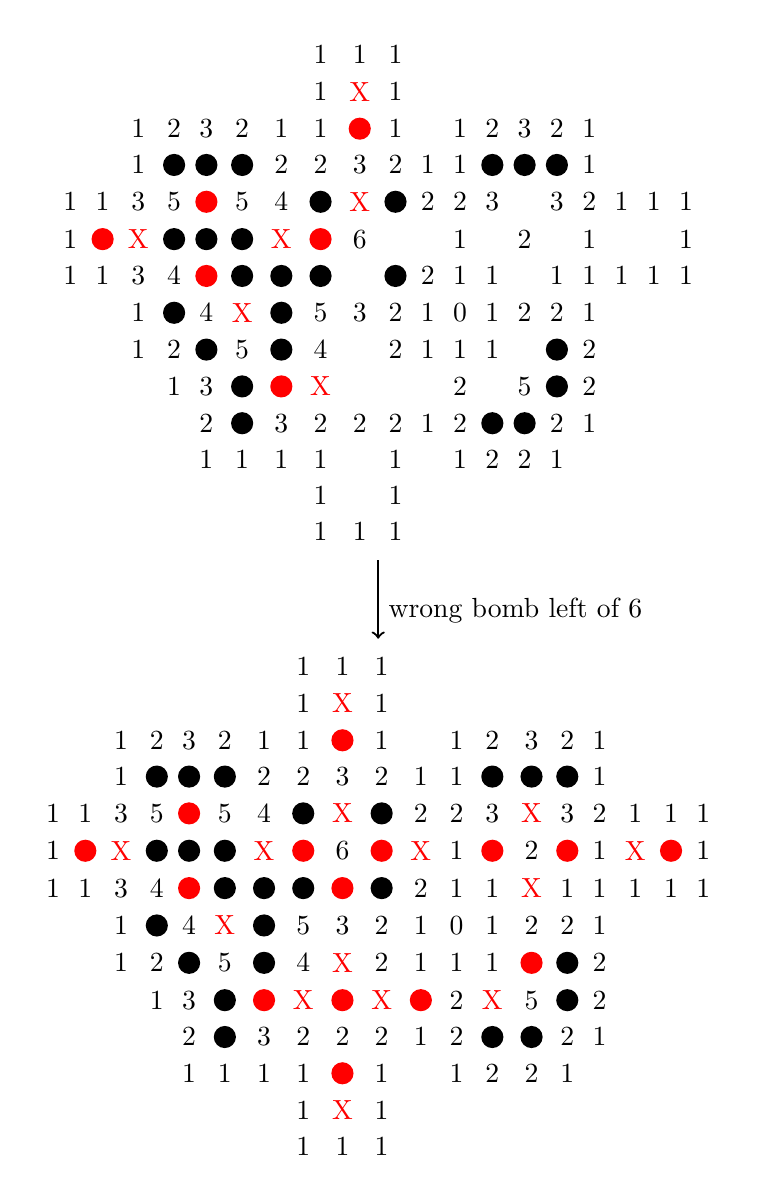
\begin{tikzpicture}
\usetikzlibrary {matrix,positioning}
    \newcommand{\greenDot}{
        \fill[color=green!70!black] circle (2pt);
    }
    \newcommand{\redDot}{
        \fill[color=red] circle (4pt);
    }
    \newcommand{\redX}{
        \node[color=red] {X};
    }
    \newcommand{\blackDot}{
        \fill[color=black] circle (4pt);
    }
  \matrix (top) [
  matrix of nodes,nodes={anchor=center}
]
  {
    &&&&&&&1&1&1&&&&&&&&& \\
    &&&&&&&1&\redX&1&&&&&&&&& \\
    &&1&2&3&2&1&1&\redDot&1&&1&2&3&2&1&&& \\
    &&1&\blackDot&\blackDot&\blackDot&2&2&3&2&1&1&\blackDot&\blackDot&\blackDot&1&&& \\
    1&1&3&5&\redDot&5&4&\blackDot&\redX&\blackDot&2&2&3&&3&2&1&1&1 \\
    1&\redDot&\redX&\blackDot&\blackDot&\blackDot&\redX&\redDot&6&&&1&&2&&1&&&1 \\
    1&1&3&4&\redDot&\blackDot&\blackDot&\blackDot&&\blackDot&2&1&1&&1&1&1&1&1 \\
    &&1&\blackDot&4&\redX&\blackDot&5&3&2&1&0&1&2&2&1&&& \\
    &&1&2&\blackDot&5&\blackDot&4&&2&1&1&1&&\blackDot&2&&& \\
    &&&1&3&\blackDot&\redDot&\redX&&&&2&&5&\blackDot&2&&&\\
    
    &&&&2&\blackDot&3&2&2&2&1&2&\blackDot&\blackDot&2&1&&&\\

    &&&&1&1&1&1&&1&&1&2&2&1&&&& \\
    &&&&&&&1&&1&&&&&&&&& \\
    &&&&&&&1&|(south)|1&1&&&&&&&&& \\
  };




\matrix (bottom)[
  matrix of nodes,nodes={anchor=center}, below=1cm of top
]
  {
    &&&&&&&1&|(north)|1&1&&&&&&&&& \\
    &&&&&&&1&\redX&1&&&&&&&&& \\
    &&1&2&3&2&1&1&\redDot&1&&1&2&3&2&1&&& \\
    &&1&\blackDot&\blackDot&\blackDot&2&2&3&2&1&1&\blackDot&\blackDot&\blackDot&1&&& \\
    
    1&1&3&5&\redDot&5&4&\blackDot&\redX&\blackDot&2&2&3&\redX&3&2&1&1&1 \\
    1&\redDot&\redX&\blackDot&\blackDot&\blackDot&\redX&\redDot&6&\redDot&\redX&1&\redDot&2&\redDot&1&\redX&\redDot&1 \\
    1&1&3&4&\redDot&\blackDot&\blackDot&\blackDot&\redDot&\blackDot&2&1&1&\redX&1&1&1&1&1 \\
    &&1&\blackDot&4&\redX&\blackDot&5&3&2&1&0&1&2&2&1&&& \\
    &&1&2&\blackDot&5&\blackDot&4&\redX&2&1&1&1&\redDot&\blackDot&2&&& \\
    &&&1&3&\blackDot&\redDot&\redX&\redDot&\redX&\redDot&2&\redX&5&\blackDot&2&&& \\
    
    &&&&2&\blackDot&3&2&2&2&1&2&\blackDot&\blackDot&2&1&&& \\

    &&&&1&1&1&1&\redDot&1&&1&2&2&1&&&& \\
    &&&&&&&1&\redX&1&&&&&&&&& \\
    &&&&&&&1&1&1&&&&&&&&& \\
  };

      \draw[thick, color=black, ->] (top.south) -- (bottom.north) node[anchor=west, yshift=10] {wrong bomb left of 6};
\end{tikzpicture}}
		\caption{Crossing Example}
		\label{fig:crossingexample}
	\end{figure}
	

	\paragraph{\textsc{\textbf{Or}}}
	A simple disjunction of the input stream of the clause and the variable input stream. The clause becomes true if it either was already true or the current literal is true. Functionally identical to a logical OR-Gate.
	
	\begin{figure}[H]
		\centering
		\scalebox{0.75}{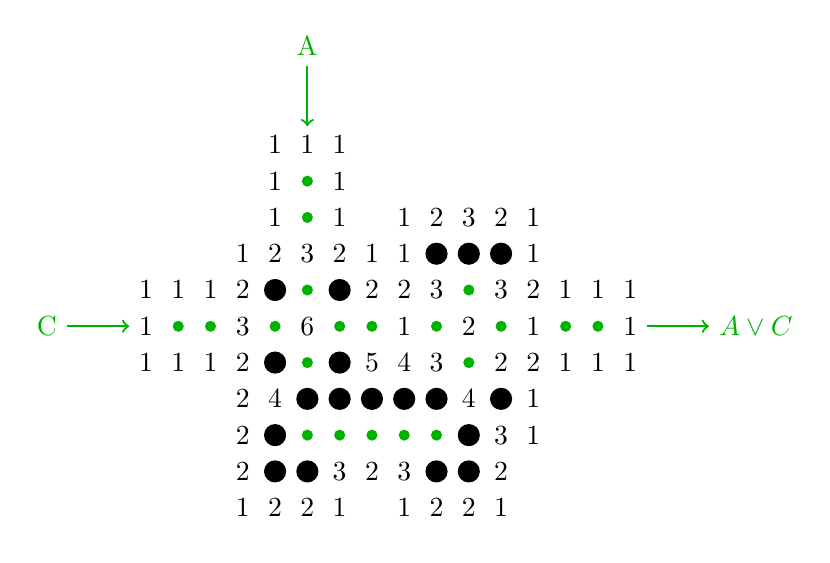
\begin{tikzpicture}
\usetikzlibrary {matrix}
    \newcommand{\greenDot}{
        \fill[color=green!70!black] circle (2pt);
    }
    \newcommand{\blackDot}{
        \fill[color=black] circle (4pt);
    }
  \matrix[
  matrix of nodes,nodes={anchor=center}
]
  {
    &&&&1&|(north)|1&1&&&&&&&&&\\
    
    &&&&1&\greenDot&1&&&&&&&&&\\
    
    &&&&1&\greenDot&1&&1&2&3&2&1&&&\\
    
    &&&1&2&3&2&1&1&\blackDot&\blackDot&\blackDot&1&&&\\
    
    1&1&1&2&\blackDot&\greenDot&\blackDot&2&2&3&\greenDot&3&2&1&1&1\\
    |(west)|1&\greenDot&\greenDot&3&\greenDot&6&\greenDot&\greenDot&1&\greenDot&2&\greenDot&1&\greenDot&\greenDot&|(east)|1\\

    1&1&1&2&\blackDot&\greenDot&\blackDot&5&4&3&\greenDot&2&2&1&1&1\\

    &&&2&4&\blackDot&\blackDot&\blackDot&\blackDot&\blackDot&4&\blackDot&1&&&\\
    &&&2&\blackDot&\greenDot&\greenDot&\greenDot&\greenDot&\greenDot&\blackDot&3&1&&&\\

    &&&2&\blackDot&\blackDot&3&2&3&\blackDot&\blackDot&2&&&&\\
    &&&1&2&2&1&&1&2&2&1&&&&\\
  };
  
\draw[thick, color=green!70!black, ->] (east) -- ++(1,0) node[anchor=west] {\(A \lor C\)};
\draw[thick, color=green!70!black, <-] (west) -- ++(-1,0) node[anchor=east] {C};
\draw[thick, color=green!70!black, <-] (north) -- ++(0,1) node[anchor=south] {A};

\end{tikzpicture}}
		\caption{Or}
		\label{fig:or}
	\end{figure}
	
	\begin{figure}[H]
		\centering
		\begin{tabular}{cc}
			\scalebox{0.6}{\input{graphics/or-a-false-c-false}} &
			\scalebox{0.6}{\input{graphics/or-a-true-c-false}} \\[1em]
			\scalebox{0.6}{\input{graphics/or-a-false-c-true}} &
			\scalebox{0.6}{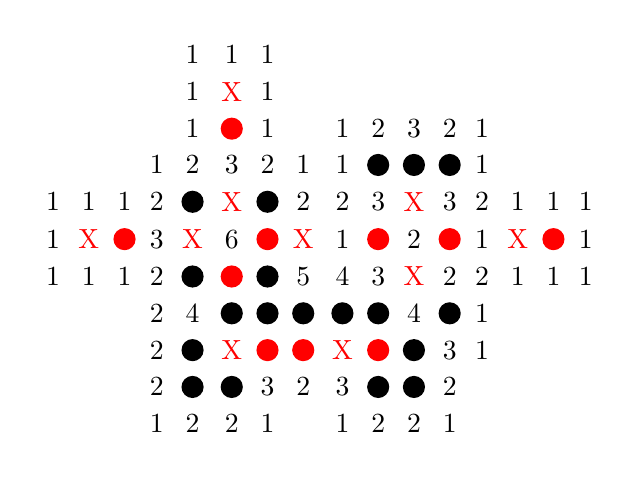
\begin{tikzpicture}
\usetikzlibrary {matrix}
   \newcommand{\redDot}{
        \fill[color=red] circle (4pt);
    }
    \newcommand{\redX}{
        \node[color=red] {X};
    }
    \newcommand{\blackDot}{
        \fill[color=black] circle (4pt);
    }
  \matrix[
  matrix of nodes,nodes={anchor=center}
]
  {
    &&&&1&1&1&&&&&&&&&\\
    
    &&&&1&\redX&1&&&&&&&&&\\
    
    &&&&1&\redDot&1&&1&2&3&2&1&&&\\
    
    &&&1&2&3&2&1&1&\blackDot&\blackDot&\blackDot&1&&&\\
    
    1&1&1&2&\blackDot&\redX&\blackDot&2&2&3&\redX&3&2&1&1&1\\
    
    1&\redX&\redDot&3&\redX&6&\redDot&\redX&1&\redDot&2&\redDot&1&\redX&\redDot&1\\

    1&1&1&2&\blackDot&\redDot&\blackDot&5&4&3&\redX&2&2&1&1&1\\

    &&&2&4&\blackDot&\blackDot&\blackDot&\blackDot&\blackDot&4&\blackDot&1&&&\\
    
    &&&2&\blackDot&\redX&\redDot&\redDot&\redX&\redDot&\blackDot&3&1&&&\\

    &&&2&\blackDot&\blackDot&3&2&3&\blackDot&\blackDot&2&&&&\\
    &&&1&2&2&1&&1&2&2&1&&&&\\
  };
  

\end{tikzpicture}}
		\end{tabular}
		\caption{Every possible assignment Clause Stream and Input Stream within Or. From top-left to bottom right the options are (Input, Clause): (false, false), (true,false), (false, true), (true, true)}
		\label{fig:orassignments}
	\end{figure}

	\paragraph{\textsc{\textbf{Splitter}}}
	This takes a variable input stream and splits it into two outputs with the same value. This is primarily used to aid us with the \textsc{\textbf{Or}} component, as otherwise we'd only have the disjunction of the clause and the literal, but this way we get to compute the variable input stream further and keep the calculation from the \textsc{\textbf{Or}} component. Thus we always use this before an \textsc{\textbf{Or}}.
	
	\begin{figure}[H]
		\centering
		\scalebox{0.6}{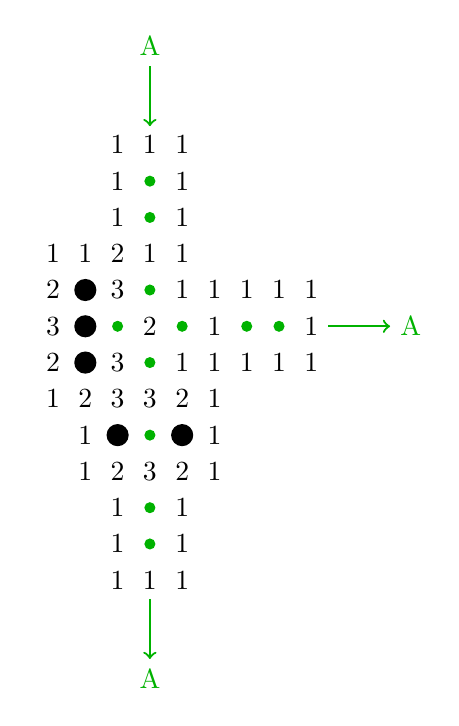
\begin{tikzpicture}
\usetikzlibrary {matrix}
   \newcommand{\greenDot}{
        \fill[color=green!70!black] circle (2pt);
    }
    \newcommand{\blackDot}{
        \fill[color=black] circle (4pt);
    }
  \matrix[
  matrix of nodes,nodes={anchor=center}
]
  {
    &&1&|(north)|1&1&&&& \\
    &&1&\greenDot&1&&&& \\
    &&1&\greenDot&1&&&& \\
    1&1&2&1&1&&&& \\
    2&\blackDot&3&\greenDot&1&1&1&1&1 \\
    3&\blackDot&\greenDot&2&\greenDot&1&\greenDot&\greenDot&|(east)|1 \\
    2&\blackDot&3&\greenDot&1&1&1&1&1 \\
    1&2&3&3&2&1&&& \\
    &1&\blackDot&\greenDot&\blackDot&1&&& \\
    &1&2&3&2&1&&& \\
    &&1&\greenDot&1&&&& \\
    &&1&\greenDot&1&&&& \\
    &&1&|(south)|1&1&&&& \\
  };
  
\draw[thick, color=green!70!black, ->] (east) -- ++(1,0) node[anchor=west] {A};
\draw[thick, color=green!70!black, <-] (north) -- ++(0,1) node[anchor=south] {A};
\draw[thick, color=green!70!black, ->] (south) -- ++(0,-1) node[anchor=north] {A};
\end{tikzpicture}
}
		
		\begin{minipage}{0.48\textwidth}
			\centering
			\scalebox{0.5}{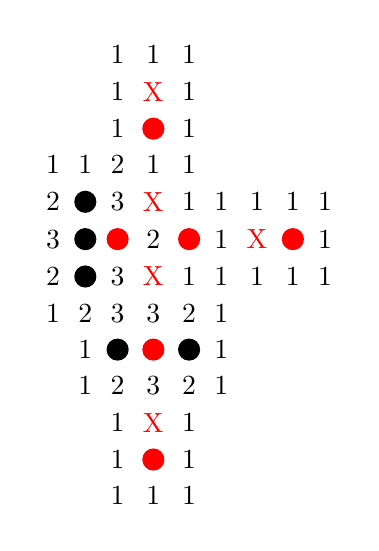
\begin{tikzpicture}
\usetikzlibrary {matrix}
   \newcommand{\redDot}{
        \fill[color=red] circle (4pt);
    }
    \newcommand{\redX}{
        \node[color=red] {X};
    }
    \newcommand{\blackDot}{
        \fill[color=black] circle (4pt);
    }
  \matrix[
  matrix of nodes,nodes={anchor=center}
]
  {
    &&1&1&1&&&& \\
    &&1&\redX&1&&&& \\
    &&1&\redDot&1&&&& \\
    1&1&2&1&1&&&& \\
    2&\blackDot&3&\redX&1&1&1&1&1 \\
    3&\blackDot&\redDot&2&\redDot&1&\redX&\redDot&1 \\
    2&\blackDot&3&\redX&1&1&1&1&1 \\
    1&2&3&3&2&1&&& \\
    &1&\blackDot&\redDot&\blackDot&1&&& \\
    &1&2&3&2&1&&& \\
    &&1&\redX&1&&&& \\
    &&1&\redDot&1&&&& \\
    &&1&1&1&&&& \\
  };
  
\end{tikzpicture}}
			\caption*{(a) true input}
		\end{minipage}
		\hfill
		\begin{minipage}{0.48\textwidth}
			\centering
			\scalebox{0.5}{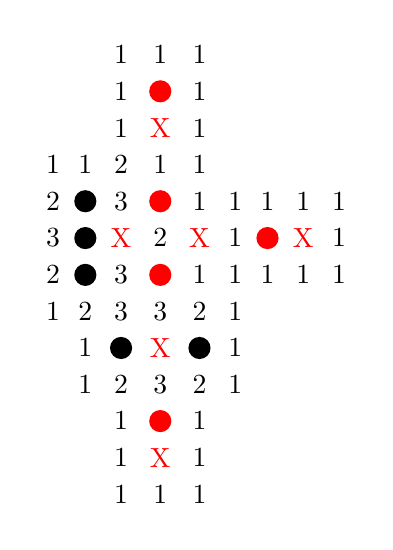
\begin{tikzpicture}
\usetikzlibrary {matrix}
   \newcommand{\redDot}{
        \fill[color=red] circle (4pt);
    }
    \newcommand{\redX}{
        \node[color=red] {X};
    }
    \newcommand{\blackDot}{
        \fill[color=black] circle (4pt);
    }
  \matrix[
  matrix of nodes,nodes={anchor=center}
]
  {
    &&1&1&1&&&& \\
    &&1&\redDot&1&&&& \\
    &&1&\redX&1&&&& \\
    1&1&2&1&1&&&& \\
    2&\blackDot&3&\redDot&1&1&1&1&1 \\
    3&\blackDot&\redX&2&\redX&1&\redDot&\redX&1 \\
    2&\blackDot&3&\redDot&1&1&1&1&1 \\
    1&2&3&3&2&1&&& \\
    &1&\blackDot&\redX&\blackDot&1&&& \\
    &1&2&3&2&1&&& \\
    &&1&\redDot&1&&&& \\
    &&1&\redX&1&&&& \\
    &&1&1&1&&&& \\
  };
  
\end{tikzpicture}}
			\caption*{(b) false input}
		\end{minipage}
		
		\caption{Splitter}
		\label{fig:splitter}
	\end{figure} 

	\paragraph{\textsc{\textbf{Turn Stream}}}
	Turns a horizontal stream into a vertical one. Needed as some components stop computing the pure input stream, but as we often still need to further process the input stream, we use this component. This module, alongside \textsc{\textbf{Splitter}}, is necessary when using the \textsc{\textbf{Or}} component. \textsc{\textbf{Turn Stream}} main functionality is that it brings both the \textsc{\textbf{Clause Stream}} and \textsc{\textbf{Input Stream}} together. Also the \textsc{\textbf{Crossing}} and \textsc{\textbf{Or}} components expect that the Input Stream is vertical.
	
	\begin{figure}[H]
		\centering
		\scalebox{0.6}{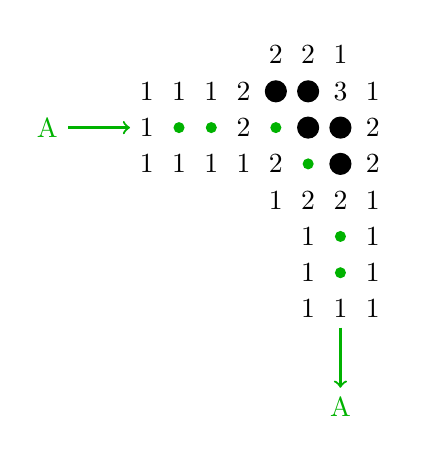
\begin{tikzpicture}
\usetikzlibrary {matrix}
    \newcommand{\greenDot}{
        \fill[color=green!70!black] circle (2pt);
    }
    \newcommand{\blackDot}{
        \fill[color=black] circle (4pt);
    }
  \matrix (M) [
  matrix of nodes,nodes={anchor=center}
]
  {
    &&&&2&2&1&\\
    1&1&1&2&\blackDot&\blackDot&3&1\\
    |(west)|1&\greenDot&\greenDot&2&\greenDot&\blackDot&\blackDot&2\\
    1&1&1&1&2&\greenDot&\blackDot&2\\
    &&&&1&2&2&1\\
    &&&&&1&\greenDot&1\\
    &&&&&1&\greenDot&1\\
    &&&&&1&|(south)|1&1\\
  };
\draw[thick, color=green!70!black, <-] (west) -- ++(-1,0) node[anchor=east] {A};
\draw[thick, color=green!70!black, ->] (south) -- ++(0,-1) node[anchor=north] {A};
\end{tikzpicture}}
		\caption{Turn Stream}
		\label{fig:turnstream}
	\end{figure} 

	\paragraph{\textsc{\textbf{Horizontal/Vertical Offset Stream}}}
	Offsets the variable \textsc{\textbf{Input Stream}} horizontally or vertically. We introduce this component as we often need to align the \textsc{\textbf{Input Stream}} after certain operations and as the input stream only repeats on every third cell.
	
	\begin{figure}[H]
		\begin{minipage}{0.48\textwidth}
			\centering
			\scalebox{0.7}{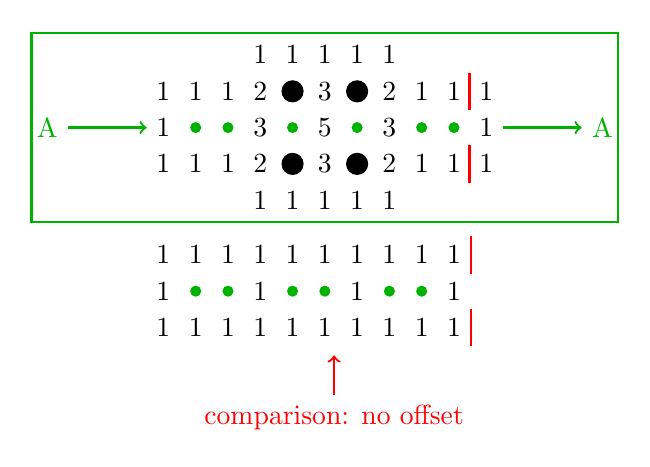
\begin{tikzpicture}
\usetikzlibrary {matrix}
\usetikzlibrary{calc}
    \newcommand{\greenDot}{
        \fill[color=green!70!black] circle (2pt);
    }
    \newcommand{\blackDot}{
        \fill[color=black] circle (4pt);
    }
  \matrix (M) [
  matrix of nodes,nodes={anchor=center}
]
  {
   &&&1&1&1&1&1&&&\\
   1&1&1&2&\blackDot&3&\blackDot&2&1&1&1\\
   1&\greenDot&\greenDot&3&\greenDot&5&\greenDot&3&\greenDot&\greenDot&1\\
   1&1&1&2&\blackDot&3&\blackDot&2&1&1&1\\
   &&&1&1&1&1&1&&&\\
   &&&&&&&&&&&&{}\\
   1&1&1&1&1&1&1&1&1&1&\\
   1&\greenDot&\greenDot&1&\greenDot&\greenDot&1&\greenDot&\greenDot&1&\\
   1&1&1&1&1&1&1&1&1&1&\\
  };
\draw[thick, color=green!70!black, <-] (M-3-1.west) -- ++(-1,0) node[anchor=east] (labelWest) {A};
\draw[thick, color=green!70!black, ->] (M-3-11.east) -- ++(1,0) node[anchor=west] (labelEast) {A};

\draw[thick, color=red] (M-2-11.north west) -- (M-2-11.south west);
\draw[thick, color=red] (M-4-11.north west) -- (M-4-11.south west);

\draw[thick, color=green!70!black] ($(labelWest) + (-0.2,1.2)$) rectangle ($(labelEast) + (0.2,-1.2)$);

\draw[thick, color=red] (M-7-10.north east) -- (M-7-10.south east);
\draw[thick, color=red] (M-9-10.north east) -- (M-9-10.south east);

\draw[thick, color=red, <-] (M.south) -- ++(0,-0.5) node[anchor=north] {comparison: no offset};

\end{tikzpicture}}
			\caption*{(a) horizontal offset}
		\end{minipage}
		\hfill
		\begin{minipage}{0.48\textwidth}
			\centering
			\scalebox{0.7}{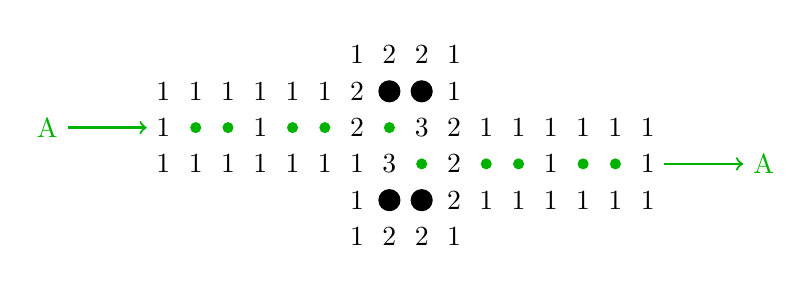
\begin{tikzpicture}
\usetikzlibrary {matrix}
\usetikzlibrary{calc}
    \newcommand{\greenDot}{
        \fill[color=green!70!black] circle (2pt);
    }
    \newcommand{\blackDot}{
        \fill[color=black] circle (4pt);
    }
  \matrix (M) [
  matrix of nodes,nodes={anchor=center}
]
  {
    &&&&&&1&2&2&1&&&&&&\\
    1&1&1&1&1&1&2&\blackDot&\blackDot&1&&&&&&\\
    1&\greenDot&\greenDot&1&\greenDot&\greenDot&2&\greenDot&3&2&1&1&1&1&1&1\\
    1&1&1&1&1&1&1&3&\greenDot&2&\greenDot&\greenDot&1&\greenDot&\greenDot&1\\
    &&&&&&1&\blackDot&\blackDot&2&1&1&1&1&1&1\\
    &&&&&&1&2&2&1&&&&&&\\
  };
  
\draw[thick, color=green!70!black, <-] (M-3-1.west) -- ++(-1,0) node[anchor=east] (labelWest) {A};
\draw[thick, color=green!70!black, ->] (M-4-16.east) -- ++(1,0) node[anchor=west] (labelEast) {A};


\end{tikzpicture}}
			\caption*{(b) vertical offset}
		\end{minipage}
		
		\caption{Offset Stream}
		\label{fig:offset}
	\end{figure} 

	\paragraph{\textsc{\textbf{Collector}}}
	This component signifies the end of a clause. All collectors have to evaluate to true, as otherwise the formula will not be satisfiable and the game field will thus also be inconsistent.
	
	\begin{figure}[H]
		\centering
		\scalebox{1.2}{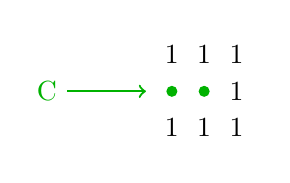
\begin{tikzpicture}
\usetikzlibrary {matrix}
   \newcommand{\greenDot}{
        \fill[color=green!70!black] circle (2pt);
    }
    \newcommand{\blackDot}{
        \fill[color=black] circle (4pt);
    }
  \matrix (M) [
  matrix of nodes,nodes={anchor=center}
]
  {
    1&1&1\\ 
    \greenDot & \greenDot &1\\
    1&1&1\\
  };

  \draw[thick, color=green!70!black, <-] (M.west) -- ++(-1,0) node[anchor=east] {C};
\end{tikzpicture}}
		
		\begin{minipage}{0.48\textwidth}
			\centering
			\scalebox{0.8}{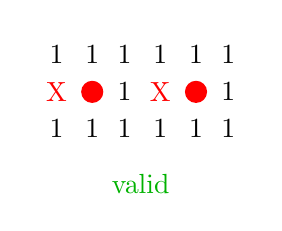
\begin{tikzpicture}
\usetikzlibrary {matrix}
   \newcommand{\redDot}{
        \fill[color=red] circle (4pt);
    }
    \newcommand{\redX}{
        \node[color=red] {X};
    }
    \newcommand{\blackDot}{
        \fill[color=black] circle (4pt);
    }
  \matrix (M) [
  matrix of nodes,nodes={anchor=center}
]
  {
    1&1&1&1&1&1\\
    \redX&\redDot&1&\redX&\redDot&1\\
    1&1&1&1&1&1\\
  };
\node[color=green!70!black, yshift=-10] at (M.south) {valid};
\end{tikzpicture}}
			\caption*{(a) true clause}
		\end{minipage}
		\hfill
		\begin{minipage}{0.48\textwidth}
			\centering
			\scalebox{0.8}{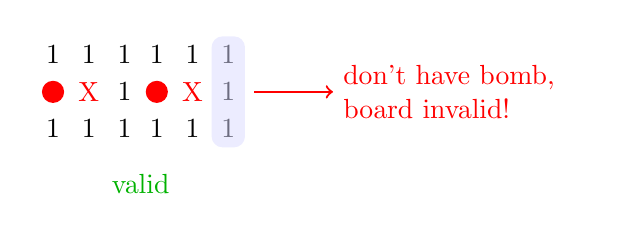
\begin{tikzpicture}
\usetikzlibrary {matrix}
   \newcommand{\redDot}{
        \fill[color=red] circle (4pt);
    }
    \newcommand{\redX}{
        \node[color=red] {X};
    }
    \newcommand{\blackDot}{
        \fill[color=black] circle (4pt);
    }
  \matrix (M) [
  matrix of nodes,nodes={anchor=center}
]
  {
    1&1&1&1&1&1\\
    \redDot&\redX&1&\redDot&\redX&1\\
    1&1&1&1&1&1\\
  };
\node[color=green!70!black, yshift=-10] at (M.south) {valid};

  \fill[blue!15,semitransparent, rounded corners]
    (M-1-6.north west)
    rectangle
    (M-3-6.south east);

\draw[thick, color=red, ->] (M.east) -- ++(1,0) node[anchor=west, text width=3cm] {don't have bomb, board invalid!};
\end{tikzpicture}}
			\caption*{(b) false clause}
		\end{minipage}
		
		\caption{Collector}
		\label{fig:collector}
	\end{figure} 

	\paragraph{\textsc{\textbf{End}}}
	Signifies the end of the variable \textsc{\textbf{Input Stream}}.
	
	\begin{figure}[H]
		\centering
		\scalebox{0.8}{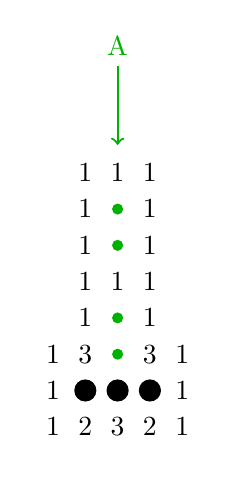
\begin{tikzpicture}
\usetikzlibrary {matrix}
    \newcommand{\greenDot}{
        \fill[color=green!70!black] circle (2pt);
    }
    \newcommand{\blackDot}{
        \fill[color=black] circle (4pt);
    }
  \matrix (M) [
  matrix of nodes,nodes={anchor=center}
]
  {
    &1&1&1&\\
    &1&\greenDot&1&\\
    &1&\greenDot&1&\\
    &1&1&1&\\
    &1&\greenDot&1&\\
    1&3&\greenDot&3&1\\
    1&\blackDot&\blackDot&\blackDot&1\\
    1&2&3&2&1\\
  };
\draw[thick, color=green!70!black, <-] (M.north) -- ++(0,1) node[anchor=south] {A};

\end{tikzpicture}}
		
		\begin{minipage}{0.48\textwidth}
			\centering
			\scalebox{0.8}{\input{graphics/end-a-true}}
			\caption*{(a) true clause}
		\end{minipage}
		\hfill
		\begin{minipage}{0.48\textwidth}
			\centering
			\scalebox{0.8}{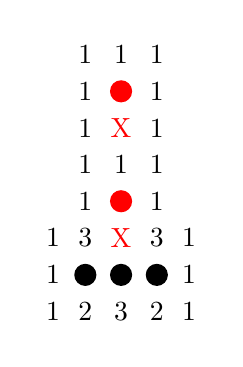
\begin{tikzpicture}
\usetikzlibrary {matrix}
       \newcommand{\redDot}{
        \fill[color=red] circle (4pt);
    }
    \newcommand{\redX}{
        \node[color=red] {X};
    }
    \newcommand{\blackDot}{
        \fill[color=black] circle (4pt);
    }
  \matrix (M) [
  matrix of nodes,nodes={anchor=center}
]
  {
    &1&1&1&\\
    &1&\redDot&1&\\
    &1&\redX&1&\\
    &1&1&1&\\
    &1&\redDot&1&\\
    1&3&\redX&3&1\\
    1&\blackDot&\blackDot&\blackDot&1\\
    1&2&3&2&1\\
  };

\end{tikzpicture}}
			\caption*{(b) false clause}
		\end{minipage}
		
		\caption{End}
		\label{fig:end}
	\end{figure} 

	\subsection{Constructing SAT Formula}
	After explaining every component within our system, we want to use them to construct a CNF formula $\varphi$. We first define a function $f: \text{\textbf{SAT}} \rightarrow \text{\textbf{MSWP}}$ that maps $\varphi$ to a game of Minesweeper.
	
	To do that we first take a look at the \textsc{\textbf{Input Stream}}. The \textsc{\textbf{Input Stream}} receives an input-dependent cell and then, depending on the value of the variable, we can determine if the input $x_i$ is a safe cell (true) or a bomb (false).
	
	Next up we analyse the \textsc{\textbf{Clause Stream}}. As defined in section \ref{sec:comp}, the \textsc{\textbf{Clause Stream}} component determines if a clause evaluate to true or not, by analysing the next literal or by taking the clauses previous state. Clauses are initialised to \textit{false} by default.
	
	Finally each clause ends up in a \textsc{\textbf{Collector}} which enforces clauses to evaluate to true. (We achieve a similar feat to that of 8.7 of the lecture script, as we have broken a large formula up into the input, consistancy and termination parts). As the size of the game board is the number of variables and clauses, the formula can be computed in polynomial time.
	
	As is immediately obvious, a constructed \textbf{MSWP} formula directly emulates a given \textbf{SAT} formula, from the literals to the clauses. Therefore any model of the formula in \textbf{SAT} directly corresponds to a model in \textbf{MSWP} (and vice versa) (\cite{MCWATER}).
	
	\subsection{3-SAT $\leq_p$ SAT}
	To also show the reduction from \textbf{3-SAT}, we will use the intermediate reduction to \textbf{SAT} (\cite{MCWATER}), the
	language of satisfiable boolean formulas in CNF.
	This relation is immediately obvious, as $\text{\textbf{3-SAT}} \subset \text{\textbf{SAT}}$.
	For the Karp reduction we have $f(x) = x$ and $x \in \text{\textbf{3-SAT}} \iff f(x) \in \text{\textbf{SAT}}$.

	\subsection{3-SAT $\leq_p$ MSWP}
	Due to the transitivity of Karp reductions, we can combine the previous reductions
	$\text{\textbf{3-SAT}} \leq_p \text{\textbf{SAT}}$ and $\text{\textbf{SAT}} \leq_p \text{\textbf{MSWP}}$ to conclude $\text{\textbf{3-SAT}} \leq_p \text{\textbf{MSWP}}$.
	
	\subsection{NP-hard \& NP-complete}
	As shown, an arbitrary formula in \textbf{3-SAT} can be converted to an instance of \textbf{MSWP} in polynomial time. This proves that MSWP is \textbf{NP}-hard.
	Together with the fact that we have proven that \textbf{MSWP} is in \textbf{NP}, we conclude that \textbf{MSWP} is \textbf{NP}-complete.

	\subsection{Cost Calculation Example}
	A \textbf{SAT} formula inside Minesweeper consists of $m$ number of clauses with $n$ amount of variables.

	If we take a $5 \times 4$ game field as an example, we can calculate the following:

	\paragraph{\textbf{Bombs}} $m \cdot (3 \cdot 98 + (n-3) \cdot 47) + n \cdot (4+4) + m \cdot (4+1)$.
	Each clause has to check three literals, all other variables not in the clause are not checked, thus we have to subtract them, Input and Output Size, Clause Start + Collector

	\paragraph{\textbf{Height}} $4 + m \cdot 25 + 5$. (Input Size, checked blocks, end size)

	\paragraph{\textbf{Width}} $4 + n \cdot 39 + 3$. (Clause Start, checked blocks, Collector Size)

	Transforming a 3-SAT Problem to a Minesweeper Problem is possible and costs are P and not exponential. Thus Minesweeper is \textbf{NP}-complete.

	\appendix

	\section{Indexes}
	\listoffigures
	\listoftables

\section{Addendum}
	This section is for interested readers who'd like to see how we derived this paper's contents.
	
	\subsection{Component Definition}
	\includepdf{../proof/Minesweeper_Component-Definition}
	
	\subsection{Cost Calculations}
	\includepdf{../proof/Minesweeper_Cost-Calculations}
	
	\subsection{Reduction to SAT}
	\includepdf{../proof/Minesweeper_to_SAT_reduction}